\makeatletter
\def\thickhrulefill{\leavevmode \leaders \hrule height 1ex \hfill \kern \z@}
\def\@makechapterhead#1{%
  \vspace*{10\p@}%
  {\parindent \z@ \centering \reset@font
        {\Huge \scshape \thechapter}
        \par\nobreak
        \vspace*{15\p@}%
        \interlinepenalty\@M
        \begin{tabular}{@{\qquad}c@{\qquad}}
          \hline
          \\
          {\Huge \bfseries #1\par\nobreak} \\
          \\
          \hline
        \end{tabular}
    \vskip 100\p@
  }}
\def\@makeschapterhead#1{%
  \vspace*{10\p@}%
  {\parindent \z@ \centering \reset@font
        {\Huge \scshape \vphantom{\thechapter}}
        \par\nobreak
        \vspace*{15\p@}%
        \interlinepenalty\@M
        \begin{tabular}{@{\qquad}c@{\qquad}}
          \hline
          \\
          {\Huge \bfseries #1\par\nobreak} \\
          \\
          \hline
        \end{tabular}
    \vskip 100\p@
  }}

\chapter{Felhasználói leírás}

\section{Hardver követelmények} % (fold)
\label{sec:hardver_követelmények}
A szoftver használatához a következő hardverekre van szükség: 
\begin{description}
  \item[Processzor] Javasolt egy legalább 1GHz Pentium CPU.
  \item[Memória (RAM)] Minimum: 1024 MB.
  \item[Merevlemez] Ruby interpreter. Rails 3.0.9. Szükséges Gem csomagok. Összesen kb. 100MB.
  \item[Monitor]  
  \item[Billentyűzet] 
  \item[Egér] 
\end{description}

Mivel ez egy webes alkalmazás, ezért platform független, azonban a következő böngészők alatt támogatott:
\begin{enumerate}
  \item Mozilla Firefox
  \item Google Chrome
  \item Openra
  \item Safari
\end{enumerate}

% section hardver_követelmények (end)

\section{Alkalmazás telepítése és indítása} % (fold)
\label{sec:alkalmazás_telepítése_és_indítása}
Sajnos a telepítés nem automatizálható teljes mértékben, ha mégis lehetséges akkor nagyon bonyolult lenne a script és felkell készíteni, hogy a következő operációs rendszereken működjön:
\begin{enumerate}
  \item Linux disztribúciók.
  \item Macintosh OSX.
  \item Microsoft Windows.
\end{enumerate}
Ezért a következő részekben tárgyalom az alkalmazás működéséhez szükséges szoftver komponenseket.
\subsection{Ruby interpreter telepítése} % (fold)
\label{sub:ruby_interpreter_telepítése}
Az alkalmazás magja, mivel a webes keretrendszer Ruby interpreteren fut.
Letölthető: \url{http://www.ruby-lang.org/en/}
Telepítési útmutatók:
\begin{enumerate}
  \item Microsoft Windows \\ \url{http://ruby.about.com/od/tutorials/a/installruby.htm}
  \item Linux \\ \url{http://ruby.about.com/od/tutorials/a/installruby.htm}
  \item Mac OSX \\ \url{http://ruby.about.com/od/tutorials/a/installruby.htm}
\end{enumerate}
% subsection ruby_interpreter_telepítése (end)

\subsection{Rails telepítése} % (fold)
\label{sub:rails_telepítése}
Miután feltelepítettük a Ruby interpretert, Ruby on Rails webes keretrendszert kell feltelepíteni.
Ezekután a Ruby csomagkezelőt kell használni, hogy feltelepítsük a Rails-t:
\begin{verbatim}
  gem install rails
\end{verbatim}
Ez a művelet eltarthat körülbelül 5-10 percig. Addig tovább mehetünk az adatbázisrendszer telepítéséez.
% subsection rails_telepítése (end)

\subsection{PostgreSQL és Postgis telepítése} % (fold)
\label{sub:postgresql_és_postgis_telepítése}
Telepítési útmutatók:
\begin{enumerate}
  \item Microsoft Windows\\
  \url{http://wiki.postgresql.org/wiki/Running_%26_Installing_PostgreSQL_On_Native_Windows}
  \item Linux \\
  \url{http://hocuspokus.net/2008/05/install-postgresql-on-ubuntu-804/}
  \item Mac OSX \\
  \url{http://macdevcenter.com/pub/a/mac/2002/06/07/postgresql.html}
\end{enumerate}
Miután felkerült a PostgreSQL adatbázisrendszer, PostGIS spatial kiegészítőt kell feltelepíteni az útmutatók alapján:
\begin{enumerate}
  \item Windows \\
  \url{http://postgis.refractions.net/download/windows/}
  \item Linux \\
  Csomag kezelő segítségével könnyen feltelepíthető.
  \item Mac OSX \\
  \url{http://www.kyngchaos.com/software:postgres}
\end{enumerate}
% subsection postgresql_és_postgis_telepítése (end)

\subsection{GeoServer telepítése} % (fold)
\label{sub:geoserver_telepítése}
Miután feltelepült a webes keretrendszer és az adatbázis rendszer. GeoServer-t, térkép szervert kell feltelepíteni.
Letölthető: \url{http://geoserver.org/display/GEOS/Download}
Azonban még mielőt nekifutnánk, JAVA JRE-t felkell telepíteni, mert a GeoServer futtatásához Java VM futtató környezet szükséges.
Letölthető: \url{http://java.com/en/download/index.jsp}
Telepítés előtt kitudjuk választani Microsoft Windows és Mac OSX-ra, hogy telepítőt használjunk vagy előre lefordított könyvtárat másoljuk be a megfelelő helyre. Linux esetében a apache web szerverre kell feltelepíteni az Geoserver-t.
Útmutatások:
\begin{enumerate}
  \item Microsoft Windows:\\
  \url{http://docs.geoserver.org/stable/en/user/installation/windows/index.html}
  \item Linux \\
  \url{http://docs.geoserver.org/stable/en/user/installation/linux/index.html}
  \item Mac OSX \\
  \url{http://docs.geoserver.org/stable/en/user/installation/osx/index.html}
  \item WAR (Web Archive) telepítés Java Application Container-be \\
  \url{http://docs.geoserver.org/stable/en/user/installation/war.html}
\end{enumerate}
% subsection geoserver_telepítése (end)

\subsection{Forráskód klónozása} % (fold)
\label{sub:forráskód_klónozása}
Mivel az alkalmazás forráskódját verziókövető rendszerben tárolom, így elérhető bárki számára a \url{https://github.com/posseidon/camapp} címen.
Letöltésére két módszer lehetséges:
\begin{enumerate}
  \item Tömörített állományban letölthető az oldalról.
  \item Git verziókövető rendszerrel klónozható a saját gépre (feltétel a GIT alkalmazás megléte).
\end{enumerate}
% subsection forráskód_klónozása (end)

\subsection{Kiegészítő Gem csomagok telepítése} % (fold)
\label{sub:kiegészítő_gem_csomagok_telepítése}
Miután az alkalmazás forráskódját sikeresen elhelyeztük a saját gépre, bekell lépni az alkalmazás könyvtárába és a következő parancsokat kell kiadni:
\begin{verbatim}
  bunlde install
  rake db:migrate
\end{verbatim}
\paragraph{bundle} parancs hatására a szükséges kiegészítő csomagokat fogja feltelepíti a Ruby csomagkezelő.

\paragraph{db:migrate} Rake parancs hatására a szükséges adatbázis szerkezetet létrehozza az adatbázisrendszerben, a \emph{database.yml} file-nak megfelelő adatkapcsolati paraméterekkel.
% subsection kiegészítő_gem_csomagok_telepítése (end)

\subsection{Alkalmazás indítása} % (fold)
\label{sub:alkalmazás_indítása}
A következő paranccsal elindítható az alkalmazás:
\begin{verbatim}
  rails server -p 8000
\end{verbatim}, ahol
\paragraph{rails server} parancs hatására elindul a webszerver.
\paragraph{-p 8000} kapcsoló definiálja, hogy melyik porton fog hallgatni a webszerver.
% subsection alkalmazás_indítása (end)
% section alkalmazás_telepítése_és_indítása (end)

\section{Alkalmazás használata} % (fold)
\label{sec:alkalmazás_használata}
Az alkalmazás három fő részből áll:
\begin{enumerate}
  \item Kamera kezelés
  \item Esemény kezelés
  \item Help
\end{enumerate}
Használatához regisztráció szükséges.

\subsection{Főoldal} % (fold)
\label{sub:főoldal}
Főodalon három link található kamera, esemény kezelésre és help oldal elérésére. Minden linkhez tartozik funkcionális linkek, amelyekre rákattintva azonnal elérhetőek a alfunkciók.

\begin{figure}[h!]
  \centering
  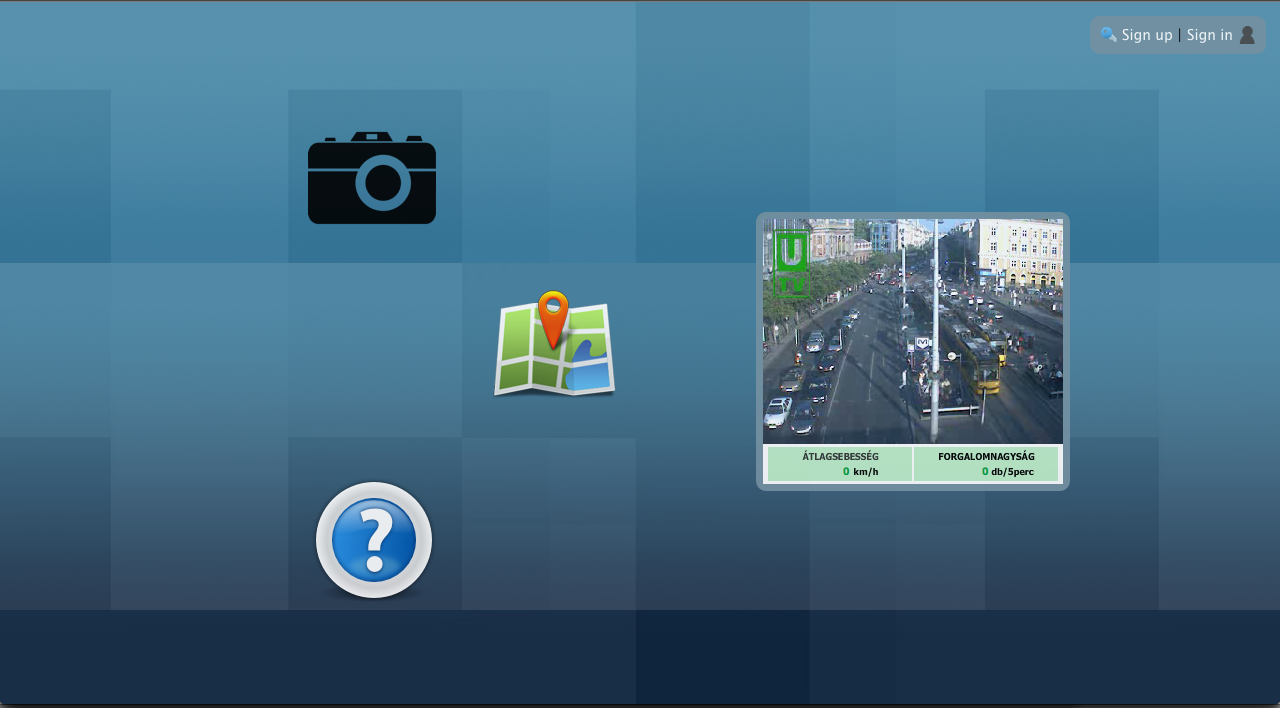
\includegraphics[width=0.8\textwidth]{chapters/chap4/main.png}
  \caption{Főoldal}
\end{figure}

Kamerához tartozó alfunkciók:
\begin{itemize}
  \item Kamerák keresés és megtekintés.
  \item Kamera felvitel.
  \item Kamera leíró adatainak módosítása.
  \item Help oldalra mutató link.
\end{itemize}

Eseményhez tartozó alfunkciók:
\begin{itemize}
  \item Események keresése és megtekintése.
  \item Esemény felvitel.
  \item Esemény leíró adatainak és geometriájának módosítása.
  \item Help oldalra muatató link.
\end{itemize}
% subsection főoldal (end)


\subsection{Bejelentkezés és regisztráció} % (fold)
\label{sub:bejelentkezés_és_regisztráció}
Jobb felső sarokban található két link regisztráció és bejelentkezésre.
Regisztráció esetén a következő adatokat kell megadni:
\begin{itemize}
  \item Email cím
  \item Jelszó
\end{itemize} 
\begin{figure}[h!]
  \centering
  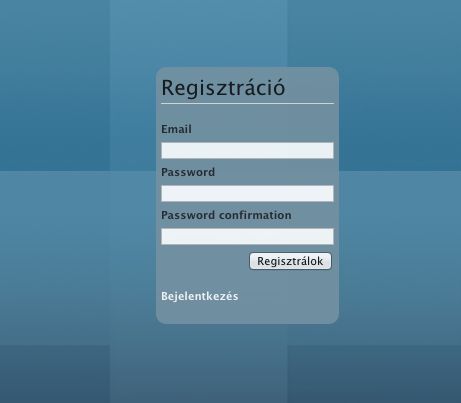
\includegraphics[width=0.5\textwidth]{chapters/chap4/register.png}
  \caption{Felhasználó regisztráció}
\end{figure}


Bejelentkezés esetén email cím és jelszó alapján történik a felhasználó azonosítás.

\begin{figure}[h!]
  \centering
  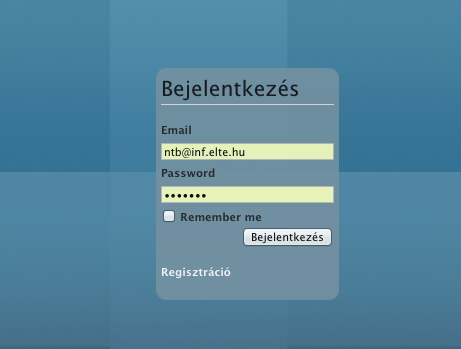
\includegraphics[width=0.5\textwidth]{chapters/chap4/login.png}
  \caption{Felhasználó bejelentkezés}
\end{figure}

% subsection bejelentkezés_és_regisztráció (end)


\subsection{Kamera nézet} % (fold)
\label{sub:kamera_nézet}
Kamerák főoldalon a következő funkciókat tartalmaz:
\begin{enumerate}
  \item Cím kereső: egy cím megadása után, az alkalmazás betölti a keresett címhez tartozó térképet.
  \item Aktív kamerák listája.
  \item Visszalépés a főoldalra.
  \item Kamera felvitel.
  \item Aktív kamerák módosítása.
  \item Aktív kamera video stream-jének megtekintése.
\end{enumerate}

\begin{figure}[h!]
  \centering
  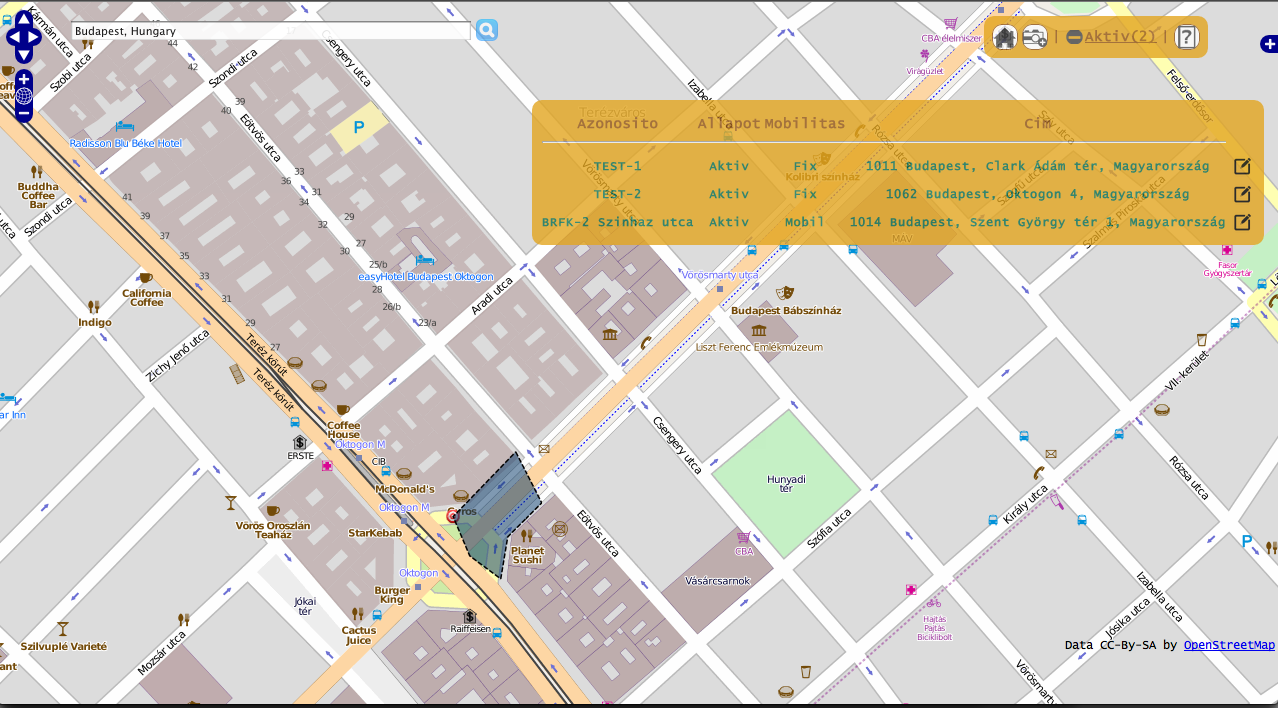
\includegraphics[width=0.5\textwidth]{chapters/chap4/cam_main.png}
  \caption{Kamera kezelés főoldal}
\end{figure}

Egy felvett kamera módosításakor a hozzátartozó geometria és leíró adatokat tudjuk módosítani.
\begin{figure}[h!]
  \centering
  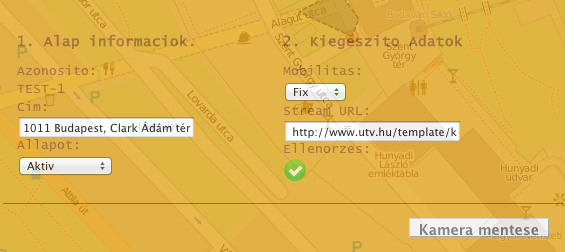
\includegraphics[width=0.5\textwidth]{chapters/chap4/cam_edit.png}
  \caption{Kamera leíró adatainak módosítási form-ja.}
\end{figure}

Geometria módosító vagy elhelyezés funkcióira vonatkozó segítség a Help oldalon található.

% subsection kamera_nézet (end)

\subsection{Esemény nézet} % (fold)
\label{sub:esemény_nézet}
Esemény főoldalon a következő funkciókat tartalmaz:
\begin{enumerate}
  \item Aktív események listája.
  \item Aktív eseményben résztvevő kamerák megtekintése.
  \item Aktív esemény módosítása.
  \item Események keresése dátum vagy azonosító alapján.
  \item Főoldalra navigálás.
  \item Help oldalra navigálás.
\end{enumerate}

\begin{figure}[h!]
  \centering
  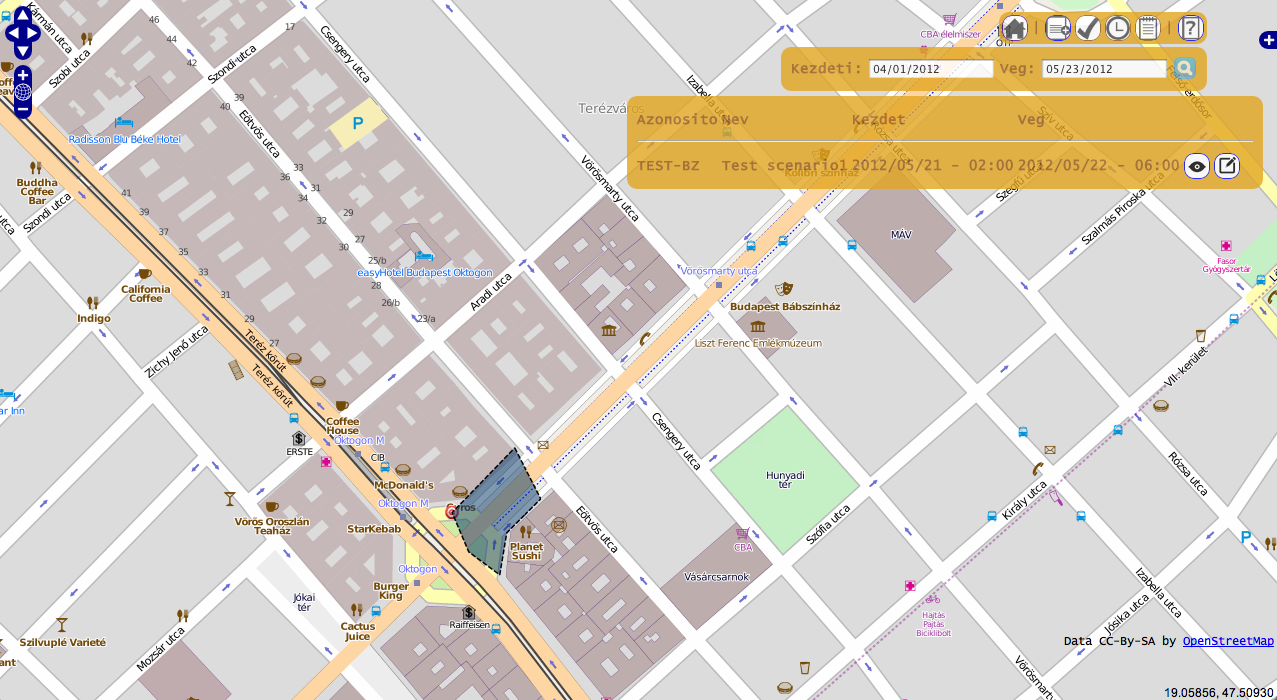
\includegraphics[width=0.5\textwidth]{chapters/chap4/scenario_main.png}
  \caption{Esemény főoldal.}
\end{figure}

Egy esemény megtekintése során résztvevő kamerák listája, kezdeti és vég dátuma, valamint a kamerákhoz tartozó státusz, mobilitás ikonok találhatóak.
Kamerák megtekintés linkre kattintva a résztvevő kamerák video stream-je jelenik meg megadott sorrendben.

\begin{figure}[h!]
  \centering
  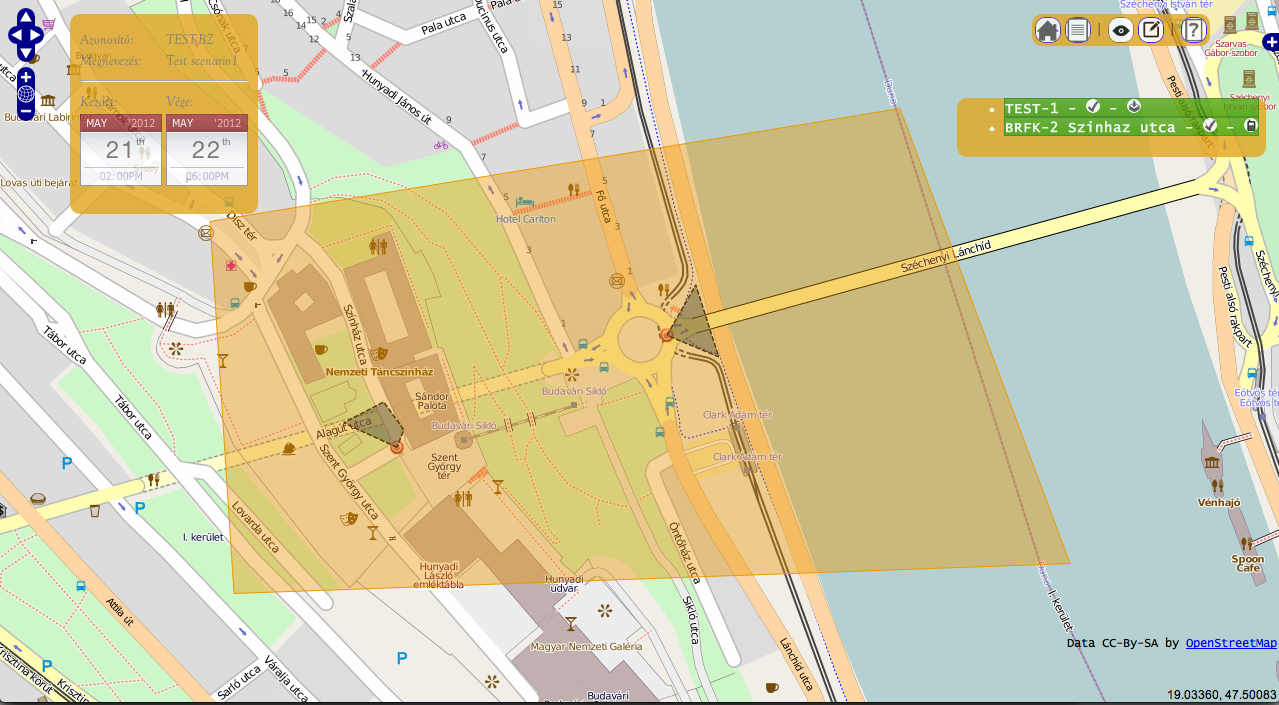
\includegraphics[width=0.5\textwidth]{chapters/chap4/scenario_view.png}
  \caption{Esemény megtekintése.}
\end{figure}

Geometria módosító vagy elhelyezés funkcióira vonatkozó segítség a Help oldalon található.

\begin{figure}[h!]
  \centering
  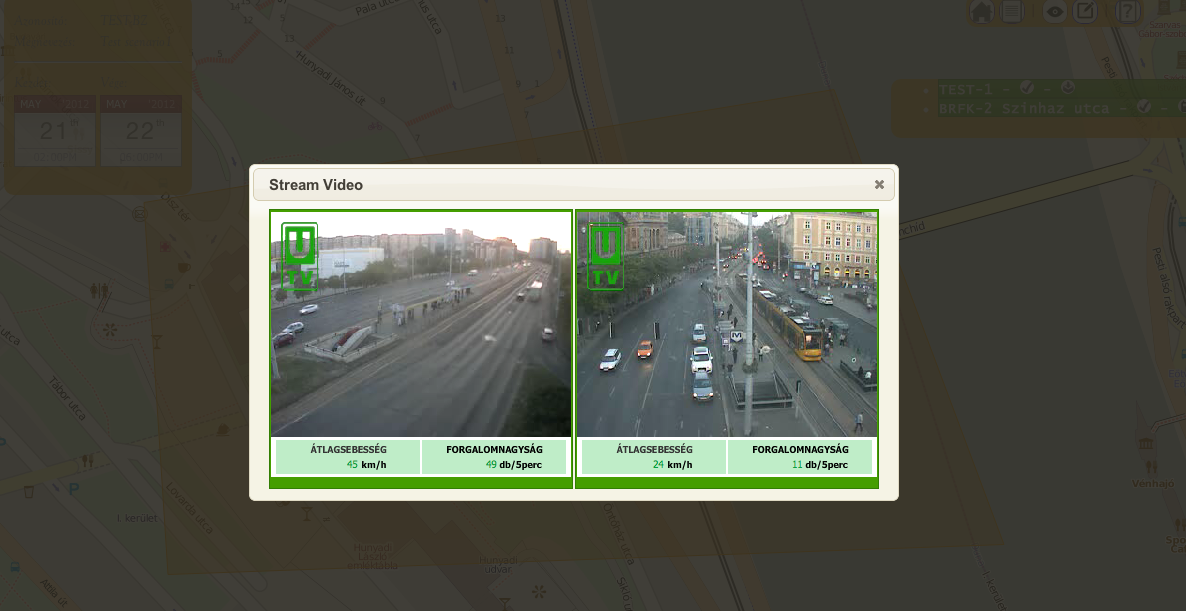
\includegraphics[width=0.5\textwidth]{chapters/chap4/scenario_cams.png}
  \caption{Eseményhez tartozó kamerák video streamje.}
\end{figure}


% subsection esemény_nézet (end)

\subsection{Help nézet} % (fold)
\label{sub:help_nézet}
Help oldalon:
\begin{itemize}
  \item Navigációs linkek.
  \item Geometria módosításához tartozó funkciók.
  \item Kamera és eseményekre vonatkozó műveletek leírása.
  \item Homokozó, ahol a felhasználó begyakorolja a térképi elemek használatát és módosítását.
\end{itemize}

\begin{figure}[h!]
  \centering
  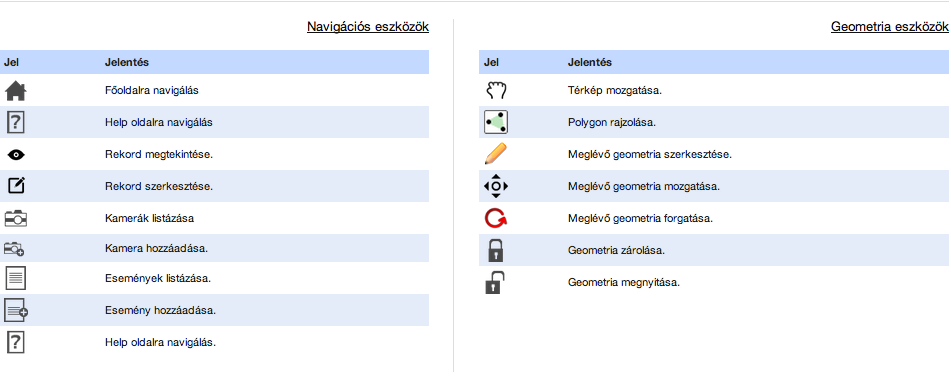
\includegraphics[width=0.5\textwidth]{chapters/chap4/help_geom.png}
  \caption{Navigációs ikonokhoz tartozó leírás.}
\end{figure}


% subsection help_nézet (end)
% section alkalmazás_használata (end)